\documentclass[12pt]{article}
\usepackage[portuguese]{babel}
\usepackage[utf8]{inputenc}
\usepackage{amsmath}
\usepackage{graphicx}
\usepackage[colorinlistoftodos]{todonotes}
\usepackage{natbib}
\usepackage{subfig}

%%---------------------------------------------------------------------------
%% New commands
%%---------------------------------------------------------------------------

%Macros para moldura preta em figuras
\newcommand{\myfboxthin}[1]{\setlength{\fboxsep}{0pt} \setlength{\fboxrule}{1.5pt} \fbox{#1}}
\newcommand{\myfbox}[1]{\setlength{\fboxsep}{0pt} \setlength{\fboxrule}{2pt} \fbox{#1}}

%Fig. references
\newcommand{\reffig}[1]{Figura~\ref{#1}}
\newcommand{\reffigp}[1]{(Figura~\ref{#1})}
\newcommand{\refsec}[1]{Seção~\ref{#1}}
\newcommand{\refchap}[1]{Capítulo~\ref{#1}}
\newcommand{\refequ}[1]{(\ref{#1})}
\newcommand{\degree}{^{\circ}}


\begin{document}

\begin{titlepage}

\newcommand{\HRule}{\rule{\linewidth}{0.5mm}} % Defines a new command for the horizontal lines, change thickness here

\center % Center everything on the page

%----------------------------------------------------------------------------------------
%	HEADING SECTIONS
%----------------------------------------------------------------------------------------

\textsc{\LARGE Universidade Federal do Rio de Janeiro}\\[1.5cm]
\textsc{\Large COE-841 Tópicos especiais em Sistemas Autônomos}\\[0.5cm] % Major heading
% such as course name
%\textsc{\large TerraMax - Oshkosh}\\[0.5cm] % Minor heading such as course
% title

%----------------------------------------------------------------------------------------
%	TITLE SECTION
%----------------------------------------------------------------------------------------

\HRule \\[0.4cm]
{ \huge \bfseries DARPA Grand Challenge 2007 -  TerraMax - Oshkosh}\\[0.4cm] %
% Title of your document
\HRule \\[1.5cm]

%----------------------------------------------------------------------------------------
%	AUTHOR SECTION
%----------------------------------------------------------------------------------------

\begin{minipage}{0.4\textwidth}
\begin{flushleft} \large
\emph{Autores:}\\
Guilherme \textsc{Carvalho} e Renan \textsc{Freitas}
\end{flushleft}
\end{minipage}
~
\begin{minipage}{0.4\textwidth}
\begin{flushright} \large
\emph{Orientador:} \\
Ramon \textsc{Costa}
\end{flushright}
\end{minipage}\\[2cm]

%----------------------------------------------------------------------------------------
%	DATE SECTION
%----------------------------------------------------------------------------------------

{\large \today}\\[2cm] % Date, change the \today to a set date if you want to be precise

%----------------------------------------------------------------------------------------
%	LOGO SECTION
%----------------------------------------------------------------------------------------


\includegraphics[height=3.5cm]{logos/ufrj-logo.png}\\[1cm]

%----------------------------------------------------------------------------------------

\vfill % Fill the rest of the page with whitespace

\end{titlepage}


%\begin{abstract}
%Your abstract.
%\end{abstract}

\section{Introdução}

O TerraMax é um veículo militar autônomo precursor de diversas tecnologias de autonomia voltada para veículos militares terrestres existentes hoje em dia. Desenvolvido pela equipe Oshkosh, o veículo participou dos desafios da DARPA (\emph{Defense Advanced Research Projects Agency}) em 2004, 2005 e 2007.

Este documento relata o desenvolvimento do veículo autônomo, com foco no desafio de 2007, o DARPA Urban Challenge, no qual o robô deve trafegar em vias urbanas respeitando leis de trânsito e cumprindo diversas manobras desafiadoras sem interferência humana. As principais informações relativas ao veículo relatadas aqui foram retiradas das referências \cite{chen2009terramax}, \cite{braid2006terramax} e \cite{broggi2008passive}.

Nesta seção introdutória, serão apresentados um breve histórico do robô, as motivações e objetivos por trás de seu desenvolvimento, a equipe desenvolvedora, e uma visão geral do veículo e o \emph{hardware} utilizado.

\subsection{Motivações e Objetivos}

O TerraMax é o único veículo, dentre todos os participantes dos DARPA \emph{Grand Challenge} (DGC) de 2004, 2005 e 2007, voltado para a aplicação militar. O objetivo da equipe Oshkosh era desenvolver tecnologia de robótica autônoma para aplicação em veículos militares terrestres com a motivação de aprimorar o suporte logístico de cargas pesadas em campos de batalha.

Tendo isso em mente, a equipe desenvolveu o robô de modo a não somente satisfazer critérios de performance nos desafios como também torná-lo apto à operação em campo. Desse modo, a escolha do \emph{hardware} e o desenvolvimento dos algoritmos de navegação considerou a aplicação militar na prática. Por exemplo, os computadores embarcados selecionados são robustos, para condições ``ultra-harsh", com encapsulamentos com certificações IP, resistência a impacto e vibração, entre outros.

Outro objetivo da equipe era desenvolver um sistema modular, de forma que novas funcionalidades poderiam ser incluídas no veículo com facilidade, e que o mesmo sistema pudesse ser utilizado para diferentes veículos militares.

\subsection{Histórico}

O TerraMax participou do desafio de 2004, em que nenhuma equipe conseguiu completar os objetivos da prova, e do DGC \emph{off-road} de 2005, antes de sua participação no DGC urbano de 2007.

A equipe realizou mudanças significativas de 2004 para 2005, como na direção das rodas traseiras para melhor desempenho em curvas acentuadas, e a completa reformulação do sistema autônomo. O TerraMax completou o desafio \emph{off-road} na quinta posição, após 28h ininterruptas de operação com sucesso em desvio de obstáculos e navegação em diferentes situações de estrada.

Para o desafio urbano, a equipe incluiu novos sensores (câmeras e LIDARs), sobretudo nas laterais e na traseira do veículo, de modo a adequar o sistema para navegação urbana. No ambiente \emph{off-road} do DCG 2005, não era necessário o sensoriamento lateral e traseiro, o que é de extrema importância no ambiente urbano para que o veículo lide com situações de ultrapassagem e cruzamentos, por exemplo.

\subsection{Equipe do DGC 2007}

Para o desafio urbano de 2007, a equipe foi incrementada com as participações da Teledyne e da Universidade de Auburn. As equipes e respectivas atribuições são descritas abaixo.

A \textbf{Oshkosh Corporation} é uma empresa americana voltada para a área de defesa, sendo a principal responsável pelo projeto. Suas atribuições no projeto foram providenciar o veículo, lidar com o gerenciamento do projeto, realizar a integração eletromecânica e o controle de \emph{software} de médio/baixo nível.

A \textbf{Teledyne Scientific and Imaging Company} é uma empresa americana de alta tecnologia voltada para pesquisa, desenvolvimento em sistemas de informação e sensoriamento de imagem para aplicações militares, espaciais e comerciais. No DGC 2007, foi responsável pelo \emph{software} de alto nível, ou seja, o comportamento autônomo do veículo, o que inclui controle de missão, planejamento de trajetórias e supervisão.

O laboratório \textbf{VisLab}, da Universidade de Parma, na Itália, continuou no projeto com a responsabilidade de desenvolver os sistemas de visão. Juntamente com os dados dos LIDARs, o sistema de visão compõe a principal parte de percepção do veículo.

A alemã \textbf{Ibeo Automotive Sensor} providenciou os LIDARs e a integração desses sensores com o \emph{software} desenvolvido para o veículo. Finalmente, a \textbf{Universidade de Auburn}, nos Estados Unidos, ficou responsável pelo desenvolvimento do sistema inercial e de GPS.

\subsection{Veículo e Visão Geral do \emph{Hardware}}

O TerraMax é uma versão adaptada de um veículo terrestre militar, um Medium Tactical Vehicle Replacement (MTVR), produzido pela Oshkosh. A equipe removeu boa parte da caçamba e o terceiro eixo de veículo, além de incluir suspensões no eixo traseiro para permitir melhor mobilidade em curvas estreitas no ambiente urbano. A \reffig{fig:veiculo} compara o veículo original com o adaptado.

\begin{figure}[h]
\centering
\subfloat{\myfboxthin{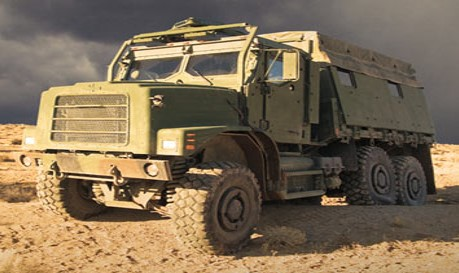
\includegraphics[height=0.375\columnwidth]{figs/MTVR.jpg}}}\enskip
\subfloat{\myfboxthin{\includegraphics[height=0.375\columnwidth]{figs/TerraMax.jpg}}}
\caption{Veículo MTVR original (esq.) e TerraMax (dir.).}%
\label{fig:veiculo}%
\end{figure}

A direção, aceleração e freio do veículo também foram adaptados para o sistema \emph{drive by wire}, e o sistema embarcado (computadores e eletrônica) foi instalado abaixo do assento do passageiro \reffigp{fig:EE}. Além disso, diversos sensores foram instalados ao redor do veículo, como será descrito mais adiante.

%Computadores
Foi utilizado um total de 6 computadores embarcados disponíveis comercialmente (\emph{commercial off-the-shelf}), além de controladores de baixo nível customizados pela Oshkosh. Dois computadores embarcados (A-Plus Mobile A20-MC) robustos e apropriados para ambientes rigorosos foram utilizados para o comportamento autônomo do veículo, rodando Windows XP como sistema operacional. Um computador SmallPC Core Duo, também com certificação IP, foi usado para cada um dos quatro sistemas de visão do veículo, rodando Linux Fedora. As Figuras \ref{fig:EE} e \ref{fig:computadores} mostram os modelos utilizados.

\begin{figure}[!h]
\centering
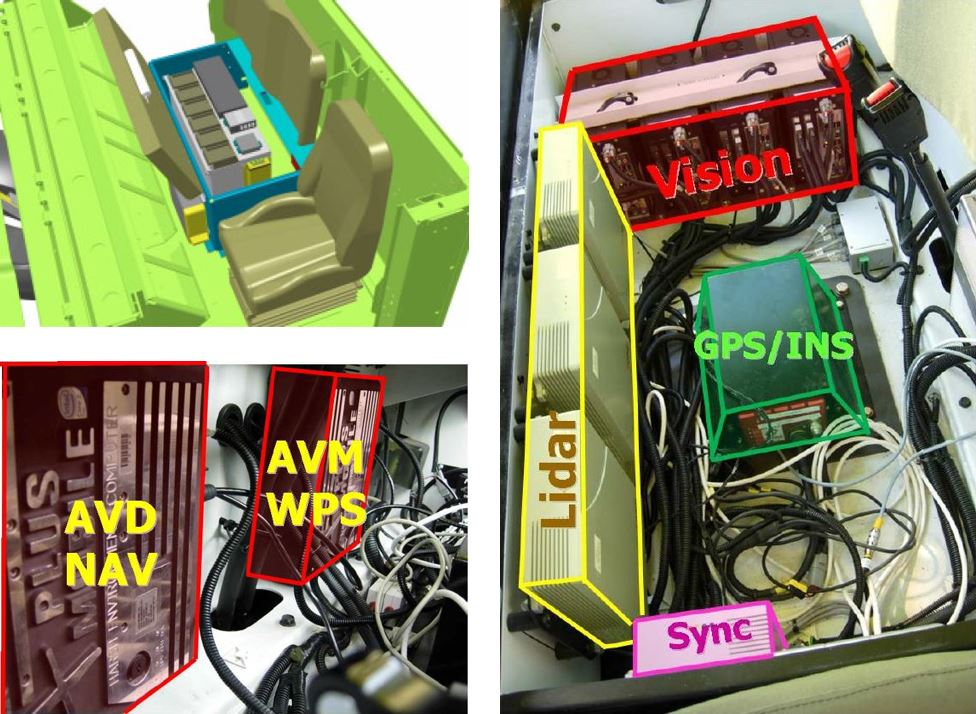
\includegraphics[width=0.75\columnwidth]{figs/EE.jpg}
\caption{Computadores embarcados robustos utilizados no TerraMax.}%
\label{fig:EE}%
\end{figure}

\begin{figure}[!h]
\centering
\subfloat{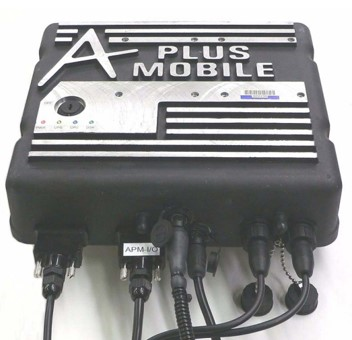
\includegraphics[height=0.375\columnwidth]{figs/Aplus.jpg}}\quad
\subfloat{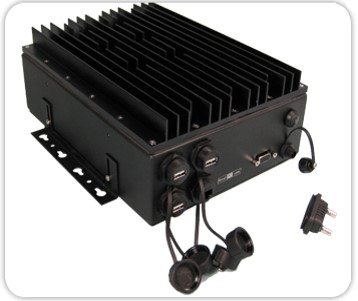
\includegraphics[height=0.375\columnwidth]{figs/SmallPC.jpg}}
\caption{Computadores embarcados robustos utilizados no TerraMax.}%
\label{fig:computadores}%
\end{figure}

O sistema de sensoriamento do TerraMax conta com 3 LIDARs (2 frontais e 1 traseiro), 11 câmeras instaladas ao redor do veículo e um sistema de navegação inercial com duas antenas GPS posicionadas na parte superior. A \reffig{fig:sensores} destaca o local de instalação desses sensores no veículo.

\begin{figure}[h]
\centering
\subfloat{\myfboxthin{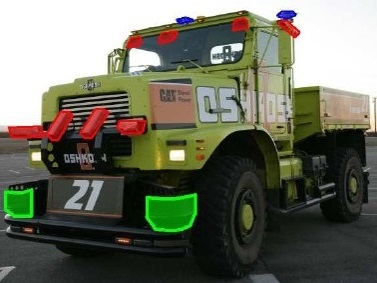
\includegraphics[height=0.3\columnwidth]{figs/front.jpg}}}\enskip
\subfloat{\myfboxthin{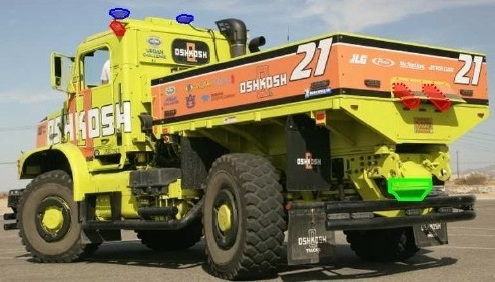
\includegraphics[height=0.3\columnwidth]{figs/rear.jpg}}}
\caption{Visão frontal e traseira do TerraMax, com destaque para os sensores instalados: câmeras (vermelho), LIDARs (verde) e antenas GPS (azul).}%
\label{fig:sensores}%
\end{figure}

Os objetivos e descrição de cada sistema de sensoriamento, bem como o hardware utilizado, serão detalhados na \refsec{sec:perception}.



\section{Sistemas de Percepção}\label{sec:perception}

\subsection{LIDAR}

O TerraMax conta com 3 LIDARs do modelo ALASCA XT da Ibeo Automotive Systems com abertura de $220\degree$ e alcance de 80m, sendo dois frontais e um traseiro, dispostos conforme mostra a \reffig{fig:lidar}. Os dois sensores frontais possuem regiões de intersecção, em que as informações são fundidas.

\begin{figure}[h]
\centering
\subfloat{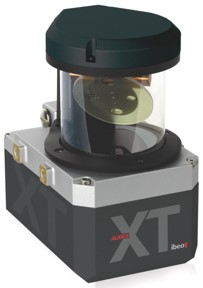
\includegraphics[height=0.35\columnwidth]{figs/lidar.jpg}}\qquad\qquad
\subfloat{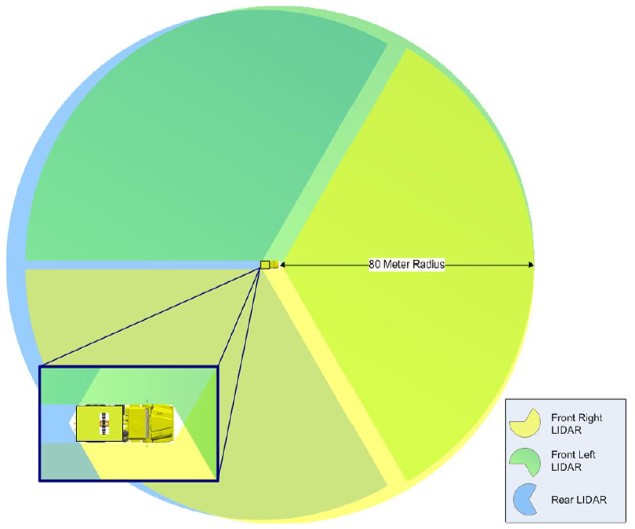
\includegraphics[height=0.35\columnwidth]{figs/laser_scan.jpg}}
\caption{Modelo de LIDAR utilizado (esq.) e região de scan (dir).}%
\label{fig:lidar}%
\end{figure}

O principal objetivo dos LIDARs é a detecção de objetos, passando essa informação já processada pelo subsistema dos LIDARs para o comportamento autônomo do sistema. Outra função é prover \emph{scans} para integração dos dados com os sistemas de imagem, aprimorando assim os resultados.

\subsection{INS}

O TerraMax utiliza um sistema de navegação inercial (INS) da Smiths Aerospace, composta por uma IMU de 6DOF integrada com informações de duas antenas GPS da Novatel e odometria das rodas em um filtro de Kalman interno \reffigp{fig:INS}. O uso de duas antenas de GPS com um baseline (distância entre as antenas) significativo de uns 2.5m aprimora as medidas de rumo da INS.

\begin{figure}[h]
\centering
\subfloat{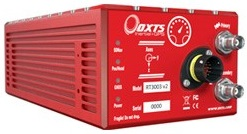
\includegraphics[height=0.25\columnwidth]{figs/INS.jpg}}\qquad
\subfloat{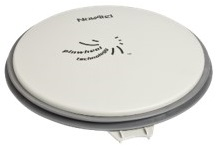
\includegraphics[height=0.25\columnwidth]{figs/antena.jpg}}
\caption{Módulo INS utilizado pelo TerraMax e uma das antenas GPS.}%
\label{fig:INS}%
\end{figure}

O objetivo da INS é naturalmente prover informações de posição absoluta no ambiente, bem como velocidades e orientações do veículo. Esses dados são utilizados no controle de trajetória juntamente com os sistemas de visão para garantir que o veículo se mantenha dentro da faixa.

Durante as etapas de teste do sistema, para efeitos comparativos da posição real do veículo com a posição estimada pelo INS, a equipe utilizou o serviço Omnistar HP, que possui precisão centimétrica.

\subsection{Sistemas de Visão}

O sistema de visão, desenvolvido pelo laboratório VisLab, é o principal sistema de percepção do TerraMax e é dividido em quatro subsistemas: trinocular, estéreo, lateral e traseiro. Ao todo, 11 câmeras foram utilizadas, sendo 9 câmeras PointGrey Flea 2 com resolução WGA (1024x768) e 2 câmeras Allied Vision Technologies Pike 2 com resolução HD (1920x1080) \reffigp{fig:cameras}.

\begin{figure}[h]
\centering
\subfloat{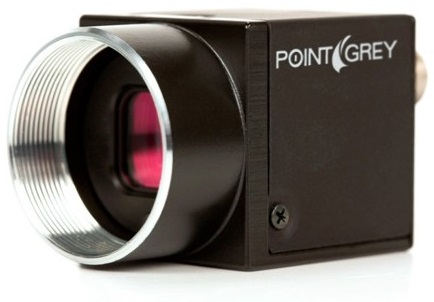
\includegraphics[height=0.25\columnwidth]{figs/Flea2.jpg}}\qquad
\subfloat{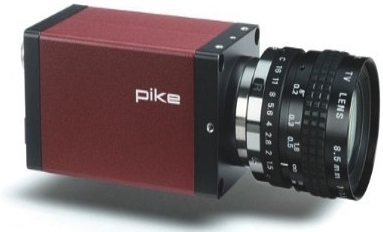
\includegraphics[height=0.25\columnwidth]{figs/Pike2.jpg}}
\caption{Câmeras utilizadas no TerraMax: Flea 2 (WGA) e Pike 2 (HD).}%
\label{fig:cameras}%
\end{figure}

As duas câmeras HD são utilizadas no sistema de visão lateral, sendo cada uma posicionada em um lado do veículo. Três câmeras são usadas no sistema trinocular, quatro no sistema estéreo (duas frontais e duas traseiras) e duas no sistema traseiro, conforme disposto na \reffig{fig:vision}.

\begin{figure}[h]
\centering
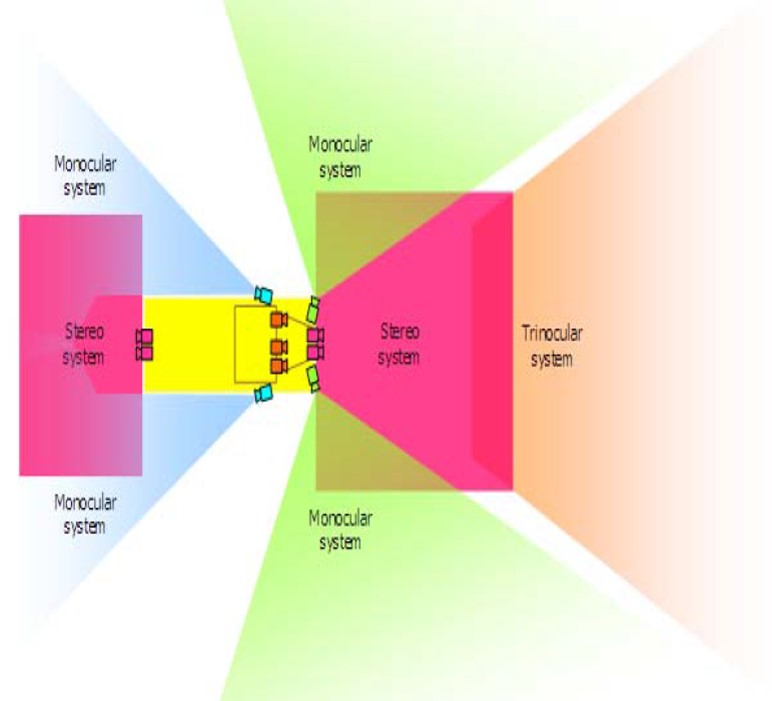
\includegraphics[width=0.75\columnwidth]{figs/vision.jpg}
\caption{Disposição das câmeras do sistema de visão.}%
\label{fig:vision}%
\end{figure}

\subsubsection{Visão Trinocular}

O sistema trinocular, que permite uma observação na faixa de 7 a 40m, é na verdade uma estratégia estéreo que pode ser chaveada em 3 diferentes \emph{baselines} (distância entre as duas câmeras). Com o veículo em velocidade baixa, é interessante utilizar o menor \emph{baseline}, mais preciso, enquanto com o veículo em alta velocidade, chaveia-se para o maior \emph{baseline}, que permite detecção de obstáculos a uma distância maior.

O objetivo desse subsistema de visão é a detecção de obstáculos à frente do veículo e a detecção das marcas da pista para controle de direção a médio e longo alcance. A escolha pelo sistema estéreo se fez porque ele permite uma reconstrução 3D do ambiente com razoável precisão sem conhecimento a priori do ambiente à frente do veículo.

O algoritmo utilizado na detecção de obstáculos inicia-se na retificação das imagens estéreo de forma a tornar as linhas epipolares horizontais, corrigindo possíveis desalinhamentos e erros de calibração das câmeras. Um mapa de disparidade ``V" extrai a inclinação da pista e do veículo para possíveis compensações durante oscilações. Então, um mapa de disparidade (diferença entre as duas imagens estéreo) é criado para realizar a detecção de obstáculos após uma filtragem da imagem correspondente ao veículo e imediatamente à sua frente. O restante do mapa de disparidade é então integrado com os scans dos LIDARs frontais para a detecção de objetos. O processo é ilustrado na \reffig{fig:trinocular_obstacle}.

\begin{figure}[h]
\centering
\subfloat[]{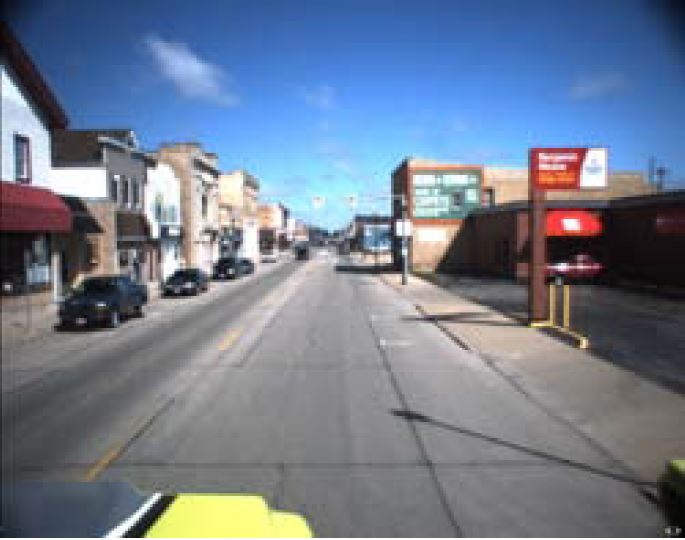
\includegraphics[height=0.275\columnwidth]{figs/trinocular_1.jpg}}\quad
\subfloat[]{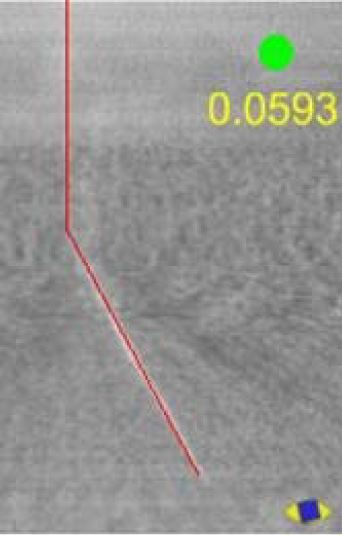
\includegraphics[height=0.275\columnwidth]{figs/trinocular_2.jpg}}\quad
\subfloat[]{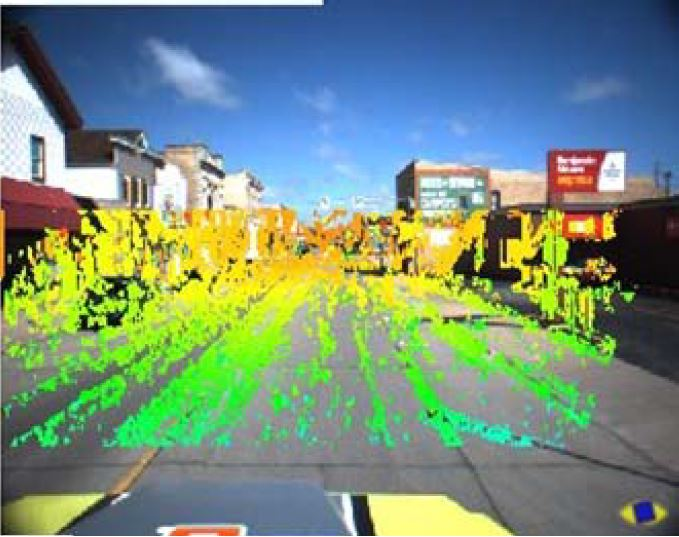
\includegraphics[height=0.275\columnwidth]{figs/trinocular_3.jpg}}
\caption{(a) Imagem original, (b) mapa de disparidade V com inclinação do veículo associada e (c) mapa de disparidade (pontos em verde próximos e em laranja mais afastados).}%
\label{fig:trinocular_obstacle}%
\end{figure}

As imagens estéreo são utilizadas também para detecção das faixas e limites das pistas. Inicialmente, a imagem é processada para remoção dos objetos detectados para diminuição de falsos positivos. Então, a imagem é duplicada e filtrada para predominância de branco em uma e amarelo na outra de modo a realizar a detecção das faixas brancas e amarelas. O efeito de perspectiva é então compensado através de uma transformação da imagem pelo mapeamento de perspectiva inversa, que leva em conta a inclinação da pista anteriormente estimada. Finalmente, é realizada uma busca de variações de luminância horizontal que permite detectar as faixas na imagem. O algoritmo possibilita detectar tanto faixas de diferente cor (amarelo e branco), como de diferente tipo (cheia ou listrada, simples ou dupla). Resultados desse processamento são mostrados na \reffig{fig:trinocular_lane}.

\begin{figure}[h]
\centering
\subfloat{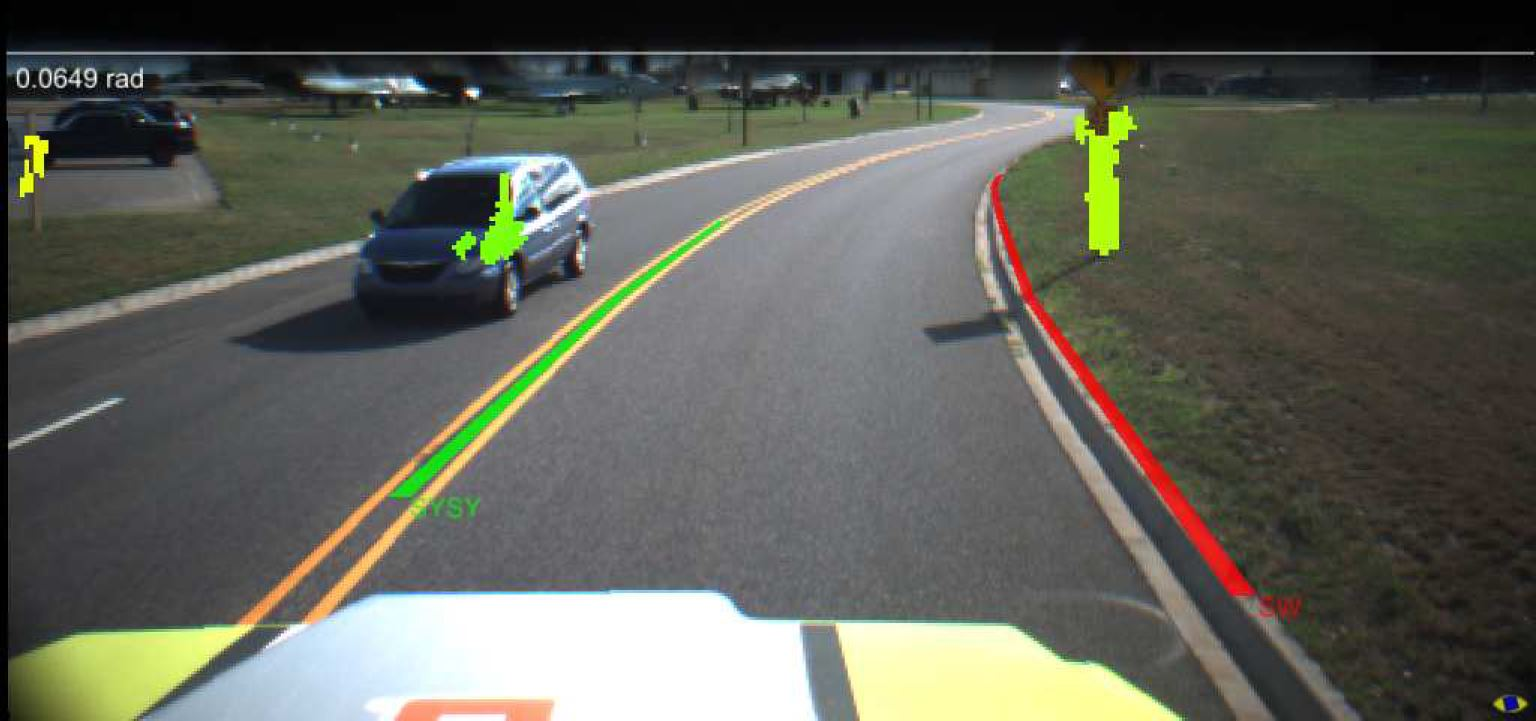
\includegraphics[height=0.225\columnwidth]{figs/trinocular_lane_2.jpg}}\quad
\subfloat{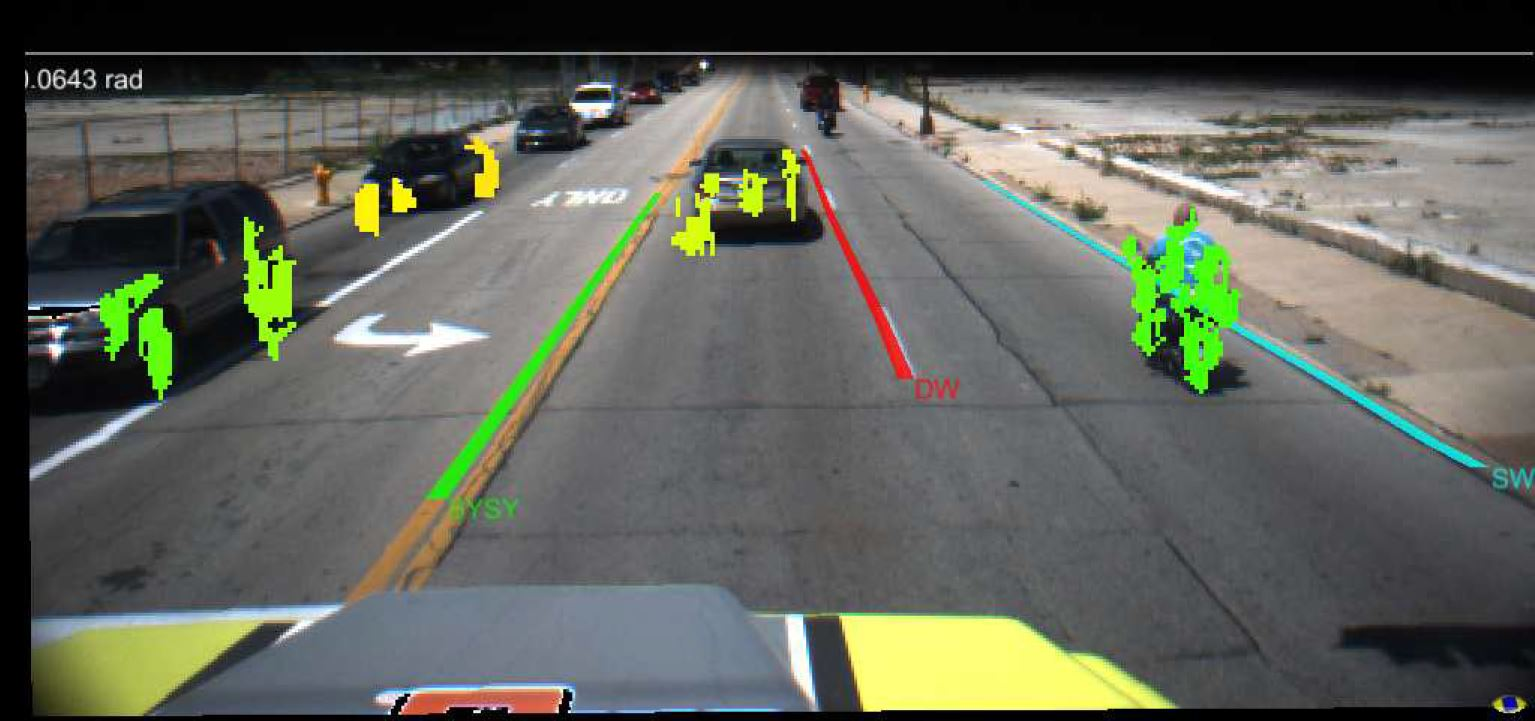
\includegraphics[height=0.225\columnwidth]{figs/trinocular_lane_3.jpg}}
\caption{Exemplos de detecção de faixas através do sistema trinocular.}%
\label{fig:trinocular_lane}%
\end{figure}

%Necessita de calibracao

\subsubsection{Visão Estéreo}

O subsistema estéreo do TerraMax possui duas câmeras frontais e duas traseiras apontadas em diagonal para o chão e possuem lentes \emph{fisheye} para ampliação do campo de visão ($\sim160\degree$) a uma área total de 10x10 metros. O objetivo é detectar obstáculos e faixas na pista próximos ao veículo com alta precisão e confiança. A ideia é aprimorar o sistema trinocular com a integração das informações dos dois subsistemas, já que faixas horizontais de parada em cruzamentos e faixas em curvas muito acentuadas não seriam detectadas pelo sistema trinocular, por exemplo.

A detecção de obstáculos é feita em dois passos. Primeiramente, as duas imagens estéreo são pré-processadas para remoção da distorção causada pela lente panorâmica e do efeito de perspectiva. Então, uma imagem diferencial é gerada e rotulada. Uma estratégia baseada em histogramas polares é utilizada para isolar os rótulos correspondentes aos obstáculos. Os dados dos LIDARs são também utilizados para melhorar a eficácia da detecção de objetos. Já a detecção de faixas utiliza a imagem de apenas uma câmera com um algoritmo semelhante ao utilizado no sistema trinocular. A \reffig{fig:stereo} mostra alguns resultados de detecção de obstáculos próximos e faixas.

\begin{figure}[h]
\centering
\subfloat{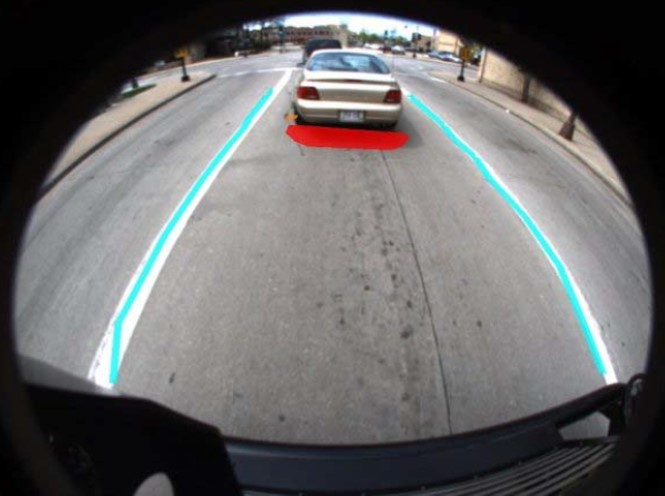
\includegraphics[height=0.235\columnwidth]{figs/stereo_1.jpg}}\quad
\subfloat{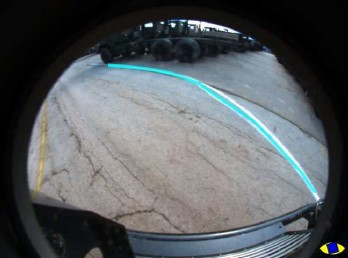
\includegraphics[height=0.235\columnwidth]{figs/stereo_2.jpg}}\quad
\subfloat{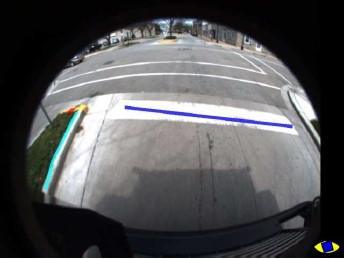
\includegraphics[height=0.235\columnwidth]{figs/stereo_3.jpg}}
\caption{Resultados de detecção de obstáculos e faixa do sistema estéreo.}%
\label{fig:stereo}%
\end{figure}

%The cameras setup selected for this system has the drawback of making it difficult to locate the exact boundaries of the detected items; to address this shortcoming, laser data is clustered and matched against the detected elements in the field of view, and when a correspondence is found the precise shape is sent to the World Perception Server. If no laser data is available, or the matching phase produces poor results, the system provides only the position of the obstacles, with no additional shape information.

\subsubsection{Visão Lateral}

O sistema de visão lateral é responsável por detectar a posição e velocidade dos veículos transitando por cruzamentos com um alcance de até 130 metros. Para reduzir o esforço computacional do processamento de imagens HD, o sistema só é ativado em situações de cruzamento. Além disso, a alta resolução é utilizada somente em determinada área de interesse, enquanto o restante é processado em uma resolução mais baixa.

A imagem é processada por um algoritmo robusto e \emph{ad-hoc} baseado em subtração de fundo em determinada região de interesse. A \reffig{fig:lateral} apresenta alguns resultados desse sistema de detecção.

\begin{figure}[h]
\centering
\subfloat{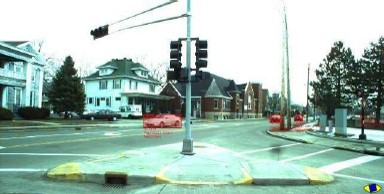
\includegraphics[height=0.24\columnwidth]{figs/lateral_1.jpg}}\quad
\subfloat{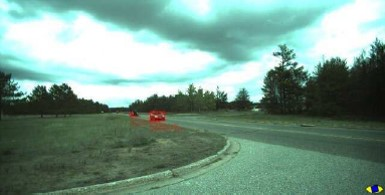
\includegraphics[height=0.24\columnwidth]{figs/lateral_2.jpg}}
\caption{Resultados de detecção de veículos pelo sistema de visão lateral.}%
\label{fig:lateral}%
\end{figure}

\subsubsection{Visão Traseira}

Através de duas câmeras instaladas na parte traseira e apontadas para trás do veículo, é possível detectar veículos que estejam fazendo ultrapassagem.

O algoritmo para detecção dos veículos é baseado em \emph{color clustering} e \emph{optical flow}. Primeiramente, porções da imagem ou objetos de cor uniforme são categorizados dependendo da cor dos pixels na imagem. Após isso, essas regiões são analisadas e rastreadas através de fluxo ótico (deslocamento de pixels ou regiões entre quadros consecutivos), estimando assim o contorno e o movimento desses objetos. As estimações também são refinadas com os dados dos LIDARs através de algoritmos de fusão sensorial. A \reffig{fig:rear} apresenta alguns resultados desse subsistema.

\begin{figure}[h]
\centering
\subfloat{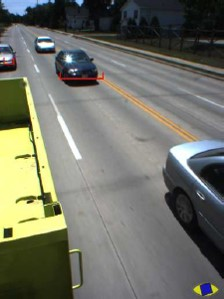
\includegraphics[height=0.3\columnwidth]{figs/rear_1.jpg}}\enskip
\subfloat{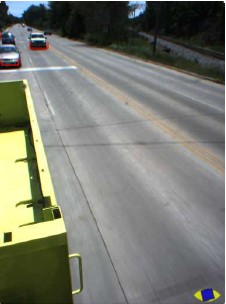
\includegraphics[height=0.3\columnwidth]{figs/rear_2.jpg}}\enskip
\subfloat{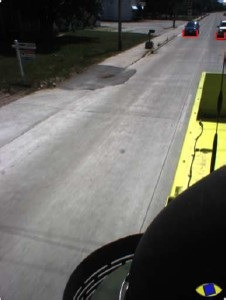
\includegraphics[height=0.3\columnwidth]{figs/rear_3.jpg}}\enskip
\subfloat{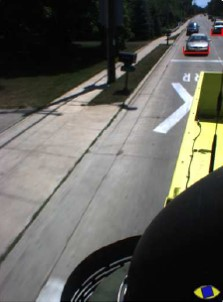
\includegraphics[height=0.3\columnwidth]{figs/rear_4.jpg}}
\caption{Resultados de detecção de veículos pelo sistema de visão traseira.}%
\label{fig:rear}%
\end{figure} 
\section{Arquitetura de sistema}

A arquitetura do sistema desenvolvido pela equipe Oshkosh pertence à classe de
arquitetura de camadas, onde cada camada depende dos dados das camadas
inferiores, não das superiores. Apesar de citado como característica comum
em sistemas de camadas, no artigo do grupo \citep{chen2009terramax}, as
dependências não necessariamente são de cima para baixo. A arquitetura de três
camadas, estado da arte das arquiteturas robóticas, utilizada por diversos
sistemas autônomos, como o AUV Phoenix \citep{gat1991reliable} e o veículo
Stanley \citep{montemerlo2006winning}, pode possuir dependências no estilo
``top-down'' ou interdependência entre camadas.

Essa arquitetura apresenta a grande vantagem de ser flexível e
modular, já que o desenvolvimento de cada camada não depende das outras e as
dependências podem ser simuladas através de objetos \textit{mock}. Com isso,
cada equipe pode trabalhar em sua especialidade, otimizando o tempo e
aumentando a qualidade dos algoritmos desenvolvidos em cada função. Vale
ressaltar que, ao fim do desenvolvimento de cada subsistema, o sistema deverá
ser integrado. Portanto, o protocolo de comunicação entre camadas e a
plataforma/framework de integração é crucial nesse tipo de arquitetura.

São apresentados sete sistemas~\ref{fig:camadas}:

\begin{enumerate}
  \item \textit{System Control and User Interface} - normalmente encontrado na
  literatura como \textit{Mission Control System}, ou planejamento de
missão (\textit{Mission Planning}) ou planejamento de tarefas (\textit{Task
Planning}). Como definido em \cite{fryxell1996navigation}, o controle de
missão é um sistema que permite ao operador definir as missões de um veículo em
linguagem de alto nível, provê ferramentas adequadas para converter planos em
Programas de Missões que podem ser verificados e executados em tempo real, e
permite ao operador saber o estado da missão enquanto esta é executada, e
modificá-la se for necessário.

  \item \textit{Autonomous Behavior} - é a parte que compõe a autonomia do robô,
  responsável pelo planejamento de trajetórias, e gerenciamento dos
  comportamentos do robô.

  \item \textit{Vehicle Management} - camada com os algoritmos de controle
  (controle de posição, estabilidade, velocidade, e  outros).

  \item \textit{Perception} - camada que possui os algoritmos de percepção, como
  detecção de obstáculos, detecção da via, detecção de tráfego, detecção de
  faixas, e outros.

  \item \textit{Sensor} - \textit{drivers} de sensores, usados para os
  algoritmos de percepção, como câmeras, LIDAR, e outros.

  \item \textit{Vehicle Status and Navigation} - sensores para o sistema de
  controle, como posição, velocidade, aceleração e estado do veículo.
\end{enumerate}

\begin{figure}[!ht]
\centering
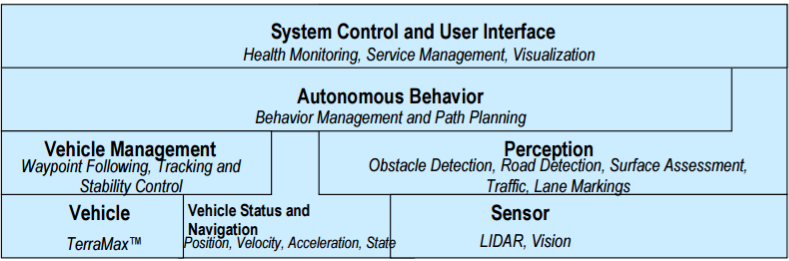
\includegraphics[width=\columnwidth]{figs/camadas.jpg}
\caption{Arquitetura de camadas do veículo TerraMax.}
\label{fig:camadas}
\end{figure}

O autor não se aprofunda, no artigo, em como é realizada a integração entre as
camadas, isto é, como a informação e dados transitam. Porém ele utiliza
uma terminologia comumente presente na literatura: ``serviços'' e
``\textit{publisher-subscriber}''. Frameworks como o ROS, estado da arte,
possibilitam a utilização de ambos os tipos de comunicação.

\begin{itemize}
  \item \textit{serviço ou cliente-servidor} -  componentes falam diretamente
  com outros componentes. As vantagens deste protocolo são: definição prévia da
  interface; e é uma abordagem distribuída para comunicação, já que não há um
  módulo central que distribui os dados. Uma desvantagem deste protocolo é o
  \textit{overhead}, que é significativo se muitos componentes precisam de uma
  mesma informação.

  \item \textit{publish-subscriber} - um componente publica dados e qualquer outro componente
pode subscrever (ouvir) a esse dado. Normalmente, há um processo central que
roteia os dados entre \textit{publish} e \textit{subscriber}. Em uma arquitetura
típica, um componente pode publicar e subscrever a vários tipos de informações.
As vantagens desse protocolo de comunicação são: simplicidade e pouco
\textit{overhead}; ideal quando não se sabe quantos componentes diferentes
necessitarão dos dados (como em muitas interfaces); componentes não ficam
sobrecarregados em caso de múltiplos pedidos de um mesmo dado. Suas principais
desvantagens são: difícil depuração de código, pois normalmente a sintaxe da
mensagem está escondida em uma simples \textit{string} (uma \textit{lista}
pode ser enviada como \textit{string} e o componente subscritor retraduz);
utilização de um servidor central que distribui as mensagens (recebe dos
\textit{publishers} e envia aos \textit{subscribers}), o que pode criar um único
ponto de falha e sobrecarga.

\end{itemize}

As camadas de \textit{System Control and User Interface} e \textit{Autonomous
Behavior} se comunicam através de mensagens do tipo serviço, enquanto que os
dados da camada \textit{Sensor} são publicados para as demais camadas.

\subsection{Autonomous Behavior}

A camada do sistema autônomo do TerraMax é desenvolvida no componente de \emph{software} chamado
\textit{Autonomous Vehicle Manager} (AVM), cujos blocos de \emph{software} estão
detalhados na Fig.~\ref{fig:avm}.

\begin{figure}[!ht]
\centering
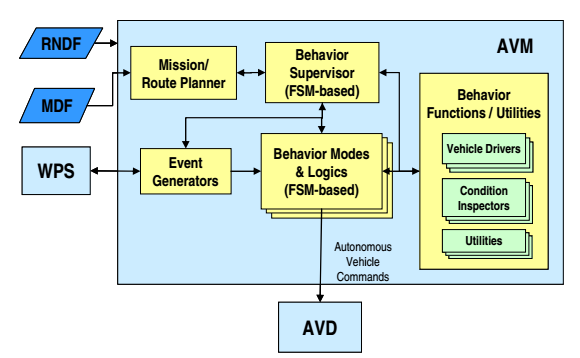
\includegraphics[width=\columnwidth]{figs/AVM}
\caption{Blocos funcionais do \textit{Autonomous Vehicle Manager}.}
\label{fig:avm}
\end{figure}

As funcionalidades de cada bloco são:

\begin{itemize}
  \item Mission Behavior Supervisor (MBS): gerencia e avalia o estado
  da missão (objetivos e sub-objetivos), seleciona e supervisiona os modos de comportamento apropriados
  para a execução;
  \item Mission Route Planner: gera rotas e planos de alto nível baseado nos
  segmentos de rota disponibilizados e zonas definidas no Road Network
  Definition File (RNDF), um arquivo disponível a todos os participantes do
  desafio, o qual contém o mapa e trechos a serem percorridos;
  \item Behavior Modes \& Logic: contém um conjunto de modos de comportamento,
  suas relações de transição e lógica de execução;
  \item Event Generators: monitora o veículo e estima o estado do ambiente pelos
  dados do WPS (dados dos sensores processados), gerando eventos apropriados
  para os modos comportamentais quando há mudanças abruptas (e.g. obstáculos);
  \item Behavior functions/utilities: provê serviços comuns para os
  comportamentos, como geração de trajetórias etc.
\end{itemize}

\subsubsection{Behavior Supervisor e Behavior Modes}

O controle supervisório adotado pela equipe do TerraMax é baseado em um sistema de
eventos discretos com Máquinas de Estado Finito (\textit{Finite State Machine},
FSM) para gerar e executar os comportamentos do veículo. Observou-se que FSM é
uma solução simples para solucionar o desafio e modela, de forma eficiente, as
regras/restrições e comportamentos/táticas do robô. Vale observar que esta é uma
estrutura hierárquica, estruturada e rígida, de forma que não é a arquitetura
ideal para ambientes extremamente dinâmicos, como é o caso da via urbana.

Apesar de usar a terminologia e ideologia de modelagem do robô em
comportamentos, a arquitetura desenvolvida não é uma arquitetura baseada em
comportamentos (Arquitetura Reativa), como aquela apresentada por
Arkin~\cite{arkin1998behavior}. Tampouco TerraMax é uma Arquitetura
Híbrida, já que o Behavior Supervisor desempenha um papel centralizador, o que
caracteriza sua arquitetura como Deliberativa.

Foram criados dezessete modos comportamentais: ChangeLane, DriveInLane,
DriveInZone, DriveToTarget, Emergent Drive, ExitParkingSpot,
InspectIntersection, InspectLaneTurn, InspectPassing, InspectUTurn,
InspectZoneIntersection, Park, Pass, PassRecovery, PerformUTurn,
RoadBlockRecovery e Wait., todos modelados como máquinas de estado finito
com parâmetros (FSMwP). Uma missão pode corresponder a um conjunto de
comportamentos, conectados logicamente, também com FSMwP. Essa conexão entre
comportamentos para executar uma missão foi chamado de Mode Transition Machine
(MTM) e corresponde a um modelo estrutural usado pelo Behavior Supervisor para a
supervisão, cuja teoria foi desenvolvida em~\cite{chen2001safety}.

Como foi comentado pelo próprio autor, o modelo de FSMwP funciona de maneira
intuitiva para a geração dos comportamentos e lógica de transição, porém sofre
dos mesmos problemas de uma arquitetura deliberativa, ou seja, robustez a
situações inesperadas e a falta de soluções criativas para a solução de
problemas, já que tudo é ``scripted''.

A fim de exemplificar esse problema, suponha que o TerraMax observe um carro
lento à frente e entre no modo de ultrapassagem. O comportamento de
ultrapassagem é a combinação dos comportamentos ``Troca de faixa", ``Dirigir
em frente", até a ultrapassagem do veículo, e ``Troca de faixa" novamente. Se
houver, porém, um segundo veículo, logo à frente do primeiro, impedindo a
segunda ``Troca de faixa'', o TerraMax terá que entrar em um sistema de
recuperação de falhas, já que este evento não havia sido pré-codificado. Observe
que há outras diversas combinações de eventos a serem considerados, o que se
torna impossível em uma arquitetura hierárquica rígida.

\subsubsection{Route planning e Trajectory planning}

O componente de \emph{software} que realiza o Route Planning do veículo TerraMax tem
por objetivo gerar uma lista ordenada dos segmentos definidos no arquivo RNDF, o
que possibilita ao veículo visitar os \textit{checkpoints} desejados, em
sequência. Os segmentos do RNDF e \textit{checkpoints} foram modelados como um
grafo, Fig.~\ref{fig:route}. O melhor caminho é computado a partir do método de
busca gulosa Dijkstra, bem conhecido na literatura \cite{cormen2001dijkstra}. O
tempo de viagem estimado foi utilizado como função custo para o método, em vez
da distância entre segmento. Essa modificação mostrou maior eficiência durante a
execução, pois levou em consideração limite de velocidade da via, condições do
tráfego, e possíveis obstáculos.

\begin{figure}[!ht]
\centering
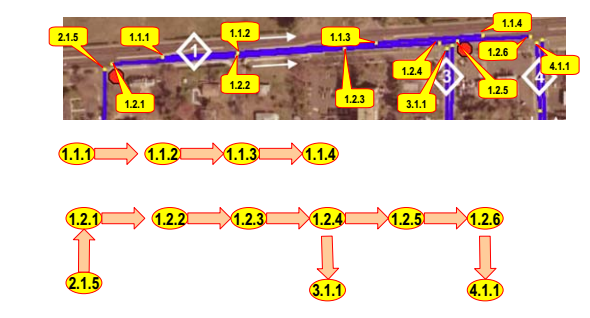
\includegraphics[width=\columnwidth]{figs/route}
\caption{Route planning modelado como um grafo de segmentos.}
\label{fig:route}
\end{figure}

Após o cálculo da melhor rota, transição dos segmentos computada pelo método de
Dijkstra, o planejador de trajetórias gera uma sequência densa e viável de
pontos objetivo (posição, \textit{waypoints}) dentro de cada segmento, com suas
correspondentes velocidades objetivo. O controle de velocidade e posição é
realizado pelo componente de \emph{software} AVD (\textit{Vehicle Status and
Navigation}), a camada funcional da arquitetura.

Foram desenvolvidos quatro tipos de \textit{trajectory planner}, os quais são
utilizados dependendo da situação em que o veículo se encontra:

\begin{itemize}
  \item \textit{Lane-following trajectory planner}: utiliza os sensores para
  detectar as bordas (meio-fio) e gera pontos objetivo no centro da via. A
  velocidade alvo é determinada considerando o espaço entre o TerraMax e o
  veículo em frente, a dinâmica do robô (e.g. velocidade atual,
  aceleração e desaceleração limite), e limite de velocidade da via.
  \item \textit{Template-base trajecotyr planners}: é um conjunto de
  planejadores que podem gerar rapidamente pontos objetivo usando padrões
  instanciados. É comum em manobras padronizadas, como troca de faixa, rotas em
  interseções e outros.
  \item \textit{Open-space trajectory planner}: provê a geração de trajetórias e
  desvio de obstáculos em um espaço aberto, isto é, ausência de via. Foi adotado
  um algoritmo similar com o A* (ou Dijkstra) após a discretização do espaço.
\end{itemize}

Os planejadores de rota e trajetória são semelhantes aos utilizados por outros
veículos do desafio e utilizam algoritmos bem consolidados na literatura.

\section{Resultados}

Esta seção é dedicada a apresentar os resultados do TerraMax no evento DGC 2007 e quais foram os principais desafios encontrados e avaliações e soluções propostas.

Anteriormente ao evento principal do DGC, os participantes foram testados em uma etapa de qualificação. Durante essa etapa, o TerraMax foi capaz de completar todas as manobras autônomas exigidas pelo desafio, tais como confluência em tráfego, cruzamentos, bloqueio de rua e retorno, ultrapassagem e estacionamento.

Alguns dos problemas já foram antecipados nesta etapa do desafio e a equipe elaborou uma lista dos problemas, causas, impactos na performance e ações de correção.

Um dos problemas foi a navegação no meio da pista devido à estreita faixa de rolamento. Por vezes, objetos próximos aos limites da pista eram detectados, e, devido ao parâmetro de segurança de distância ao limite da pista, o robô acabou andando no meio da via urbana. A ação de correção tomada foi diminuir o parâmetro de segurança e a lição aprendida foi que é realmente difícil navegar com um veículo de grande porte em uma via urbana.

Outro problema apontado foi o de uma nuvem de poeira criada pelo próprio veículo em manobras bruscas de frenagem. Essa nuvem compromete tanto os sistemas de visão como os LIDARs para detecção de obstáculos, criando falsos positivos (nuvem de poeira detectada como obstáculo) fazendo o veículo parar e demorar mais a completar a missão, esperando a poeira baixar.

Um terceiro problema a destacar foi a oclusão de obstáculos, como um veículo sendo ocluso por outro em um cruzamento. Isso levou à tomada errada de decisões em situações de cruzamento e a equipe tentou corrigir o problema aprimorando o sistema de rastreamento dos veículos por visão e a fusão sensorial entre visão e \emph{laser scans}.

Um erro em um dos LIDARs também causou problemas ao robô, que quase colidiu com um veículo à sua frente. O erro foi corrigido, mas ficou a lição de que redundância é importante em veículos autônomos.

Durante o evento principal, o robô autônomo completou as primeiras quatro sub-missões com sucesso, porém parou na parte do estacionamento devido a um problema de \emph{software}. O robô realizou a manobra de entrada e saída da vaga de estacionamento normalmente. Porém, após sair da vaga, o planejador de trajetórias, devido a um \emph{bug} de \emph{software}, produziu \emph{waypoints} duplicados, resultando em uma paralisação do veículo por 17 minutos.

Após esse tempo, a estimação da posição do veículo pelo GPS derivou e levou à geração de 4 \emph{waypoints} em modo de espaço aberto pelo planejador de trajetórias. Sendo assim, o comportamento autônomo do veículo comandou-o para acelerar em linha reta em direção ao muro do estacionamento. O veículo tornou-se irresponsivo a novos comandos do sistema autônomo, continuando a se mover em direção ao muro, e teve que ser parado por situação de emergência pelos organizadores do desafio.

A equipe do TerraMax testou extensivamente o sistema novamente no mês seguinte ao desafio após as correções de falhas de \emph{software}, porém sem atualização de versão. Com um tempo total de teste de 8h e 125Km dirigidos com uma velocidade média de 16Km/h, o TerraMax obteve uma taxa de falha de 6.25\% (7 falhas em 112 sub-missões).





\section{Conclusões}

O TerraMax foi o único veículo realmente voltado a aplicações militares de logística dentre os participantes do desafio financiado pela agência de defesa americana. O sistema obteve resultados relativamente satisfatórios durante a fase de desenvolvimento e mesmo durante a competição, sendo capaz de realizar várias manobras complexas autonomamente.

No entanto, dados os problemas apresentados durante as etapas de teste e a performance no desafio principal, ficaram evidentes algumas limitações do robô frente a situações não previstas, como já apontado neste relatório. A lição aprendida é que robustez e resiliência são essenciais em sistemas autônomos.

Apesar de não ter completado a prova no evento final do DARPA Grand Challenge 2007, o TerraMax foi de fundamental importância para impulsionar o desenvolvimento de tecnologias de robótica autônoma, principalmente voltadas à aplicação militar.


%\todo{Here's a comment in the margin!}
%
%\todo[inline, color=green!40]{This is an inline comment.}

%\subsection{Tables and Figures}

\bibliography{main}

\end{document} 